\documentclass[a4paper,12pt]{exam}
	\usepackage{graphicx}
	\usepackage[utf8]{inputenc}
	\usepackage[T1]{fontenc}
	\usepackage{listings}
	\usepackage{color}
	\usepackage{amsmath}
	\usepackage{enumerate}
	\usepackage{caption}
	\usepackage{subcaption}
	\definecolor{dkgreen}{rgb}{0,0.6,0}
	\definecolor{gray}{rgb}{0.5,0.5,0.5}
	\definecolor{mauve}{rgb}{0.58,0,0.82}

	\lstset{frame=tb,
	  language=Python,
	  aboveskip=3mm,
	  belowskip=3mm,
	  showstringspaces=false,
	  columns=flexible,
	  basicstyle={\small\ttfamily},
	  numbers=none,
	  numberstyle=\tiny\color{gray},
	  keywordstyle=\color{blue},
	  commentstyle=\color{dkgreen},
	  stringstyle=\color{mauve},
	  breaklines=true,
	  breakatwhitespace=true
	  tabsize=3
	}

\begin{document}
\begingroup 
	  \bf \Large Mecânica Clássica I\\
	  \indent \normalsize André Del Bianco Giuffrida
	\endgroup
	\\ \quad
	\\
	A distância do Perielio ao sol do planeta Marte é de $2,06\times 10^8 km$, já a distância do afélio é de $2,485 \times 10^8 km$.
	Suponha que a órbita da terra está no mesmo plano e é circular de raio $1,49 \times 10^8 km$ e o período de 1 ano. Determine com esses dados a velocidade de Marte no Periélio.
	
	Primeiramente vamos escrever a orbita dos dois:
	\[ r_{Marte}(\theta) = \frac{a(1-\epsilon^2)}{1+\epsilon\cos{(\theta)}}\]
	\[r_{Terra}(\theta) = cte\]
		\begin{figure}[h]
			\centering
			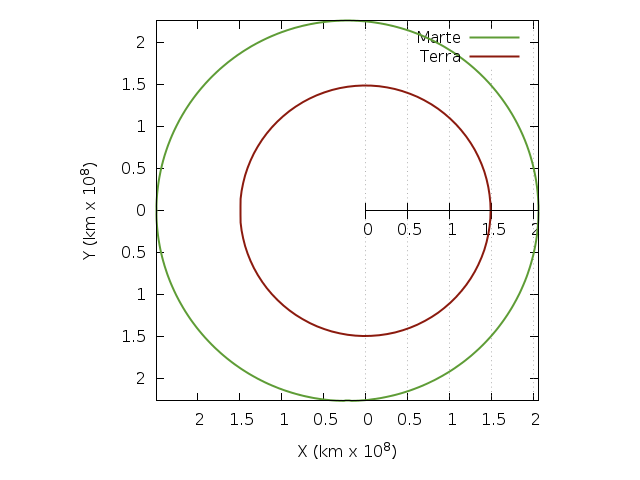
\includegraphics[scale=0.6]{6o0.png}
			\caption{Orbitas}
		\end{figure}
	
	Segundo Kepler \textit{"Os quadrados dos períodos de translação dos planetas são proporcionais aos cubos dos semi-eixos maiores de suas órbitas".} 
	\[ \frac{(2 \pi / \dot\theta_{Marte})^2}{((2,06 + 2,485)\times 10^8)^3}= \frac{\text{ano}^2}{(2,98 \times 10^8)^3}\]
	E assim obtemos o período de Marte:
	\[\frac{1}{ \dot\theta_{Marte} }= \sqrt{\frac{(2,06 + 2,485)^3}{(2,98)^3} } \frac{\text{ ano}}{2\pi}\]
	\[ \dot\theta_{Marte} = \frac{2\pi}{1,88 \text{ano}}\]
	Para calcular a velocidade de Marte no periélio basta lembrar que $\vec{v} = \dot r \hat r + r\dot\theta \hat\theta$
	podemos ver que $\dot r = 0$ quando $\theta = 0$ pois:
	\[\frac{d}{dt}r(\theta) = \dot r(\theta) = \frac{a(1-\epsilon^2) sin(\theta) \dot\theta}{(1+\epsilon\cos{(\theta)})^2} \]
	\[ \dot r(0) = 0 [km/ano] \hat r\]
	já na direção $\hat \theta$ temos:
	\[ r_{perielio}\dot\theta_{Marte} = 2,06 \times 10^8 \frac{2\pi}{1,88} [km/ano] \]
	\[v = 6,8847 \times 10^8[km/ano] = 7,859 \times 10^{4} [km/h]\]
	
	
		
	\end{document}
